\documentclass[tikz,border=5pt]{standalone}
\usepackage{amsmath}
\usetikzlibrary{arrows.meta}

\begin{document}
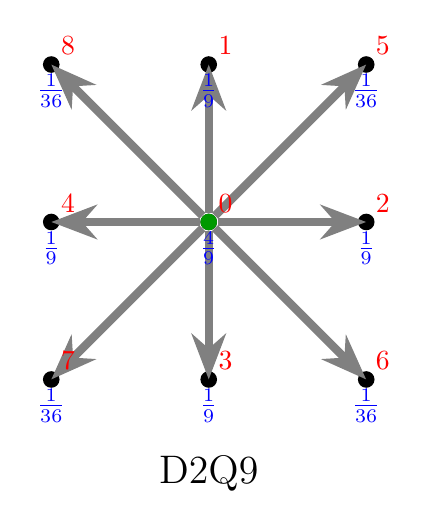
\begin{tikzpicture}[scale=2,>=Stealth]

    % 定义节点位置
    \foreach \x in {0,1,2} {
            \foreach \y in {0,1,2} {
                    \node[circle,fill=black,minimum size=6pt,inner sep=0pt] (n\x\y) at (\x,\y) {};
                }
        }

    % 中心绿色节点
    \node[circle,fill=green!60!black,minimum size=6pt,inner sep=0pt] (center) at (1,1) {};

    % 八个方向的短箭头(半透明)
    \foreach \dx/\dy in {-1/0,1/0,0/-1,0/1,-1/-1,1/-1,-1/1,1/1} {
            \draw[gray,->,line width=3pt] (center) -- ++(\dx,\dy);
        }

    \node[blue,anchor=north] at (0,0) {$\frac{1}{36}$};
    \node[blue,anchor=north] at (0,1) {$\frac{1}{9}$};
    \node[blue,anchor=north] at (0,2) {$\frac{1}{36}$};

    \node[blue,anchor=north] at (1,0) {$\frac{1}{9}$};
    \node[blue,anchor=north] at (1,1) {$\frac{4}{9}$};
    \node[blue,anchor=north] at (1,2) {$\frac{1}{9}$};

    \node[blue,anchor=north] at (2,0) {$\frac{1}{36}$};
    \node[blue,anchor=north] at (2,1) {$\frac{1}{9}$};
    \node[blue,anchor=north] at (2,2) {$\frac{1}{36}$};

    \node[red,anchor=south west] at (0,0) {7};
    \node[red,anchor=south west] at (0,1) {4};
    \node[red,anchor=south west] at (0,2) {8};

    \node[red,anchor=south west] at (1,0) {3};
    \node[red,anchor=south west] at (1,1) {0};
    \node[red,anchor=south west] at (1,2) {1};

    \node[red,anchor=south west] at (2,0) {6};
    \node[red,anchor=south west] at (2,1) {2};
    \node[red,anchor=south west] at (2,2) {5};

    % 底部普通字体 D2Q9
    \node[font=\Large] at (1,-0.6) {D2Q9};

\end{tikzpicture}
\end{document}
